\documentclass{llncs}
\usepackage[utf8]{inputenc}
\usepackage[spanish,es-tabla]{babel}
\usepackage{graphicx}
\usepackage{amsmath}
\usepackage{booktabs}
\usepackage{hyperref}
\usepackage{float}
\usepackage{adjustbox}
\usepackage{subcaption}

% Traducción de términos al español
\renewcommand{\abstractname}{Resumen}
\renewcommand{\refname}{Referencias}
\renewcommand{\figurename}{Figura}
\renewcommand{\tablename}{Tabla}

% Configurar fecha en español
\addto\captionsspanish{%
  \def\today{\number\day\space de \ifcase\month\or
    enero\or febrero\or marzo\or abril\or mayo\or junio\or
    julio\or agosto\or septiembre\or octubre\or noviembre\or diciembre\fi
    \space de \number\year}%
}

\begin{document}
\title{Clasificación de Lesiones Cutáneas mediante Aprendizaje Profundo con YOLO}

\author{Alejandro Cerezo, Germán Torres y Daniil Nemchenko}

\maketitle

\begin{abstract}
En este trabajo presentamos un sistema de clasificación de lesiones cutáneas basado en aprendizaje profundo utilizando la arquitectura YOLO (You Only Look Once). Hemos trabajado con el conjunto de datos ISIC 2019, que contiene imágenes dermatoscópicas de ocho tipos diferentes de lesiones de la piel, incluyendo melanoma, nevus, carcinoma basocelular, queratosis actínica, queratosis benigna, dermatofibroma, lesiones vasculares y carcinoma de células escamosas. Entrenamos tres variantes del modelo YOLOv8, específicamente las versiones nano, small y medium, utilizando un subconjunto de 100 imágenes por clase para entrenamiento y 10 imágenes por clase para evaluación. Nuestros resultados muestran que el modelo YOLOv8m alcanza el mejor rendimiento con un mAP50 de 0.664 y un mAP50-95 de 0.661, mientras que el modelo YOLOv8s obtiene la mayor accuracy en clasificación con 0.633. El análisis de las curvas de entrenamiento revela que nuestros modelos no presentan sobreajuste significativo y que las versiones más grandes de YOLO proporcionan mejoras graduales en el rendimiento a costa de mayor tiempo de inferencia.
\end{abstract}

\section{Introducción}

El cáncer de piel representa uno de los tipos de cáncer más frecuentes a nivel mundial, y la detección temprana de lesiones malignas como el melanoma resulta fundamental para mejorar el pronóstico de los pacientes. En este contexto, las técnicas de aprendizaje profundo han demostrado un potencial extraordinario para asistir a los dermatólogos en el diagnóstico de lesiones cutáneas a partir de imágenes dermatoscópicas. La capacidad de las redes neuronales convolucionales para extraer características relevantes de las imágenes de forma automática ha revolucionado el campo de la visión por computador aplicada a la medicina.

En este proyecto hemos trabajado con el conjunto de datos ISIC 2019 (International Skin Imaging Collaboration), que constituye uno de los recursos más completos y utilizados en la investigación sobre clasificación de lesiones cutáneas. Este dataset contiene miles de imágenes dermatoscópicas etiquetadas con ocho categorías diagnósticas diferentes que abarcan desde lesiones benignas como el nevus hasta lesiones malignas como el melanoma y el carcinoma de células escamosas.

Nuestro objetivo principal ha sido entrenar modelos de detección de objetos basados en la arquitectura YOLO (You Only Look Once) para clasificar imágenes de lesiones cutáneas. Hemos elegido YOLO por su eficiencia en tiempo real y su capacidad para procesar imágenes de forma rápida sin sacrificar significativamente la precisión. Aunque YOLO fue diseñado originalmente para detección de objetos, hemos adaptado su uso para el problema de clasificación de imágenes médicas, aprovechando su arquitectura de red neuronal convolucional profunda.

Hemos entrenado tres variantes del modelo YOLOv8, correspondientes a las versiones nano (n), small (s) y medium (m), con el propósito de analizar el compromiso entre complejidad del modelo, tiempo de entrenamiento y rendimiento final. Para cada modelo, hemos generado gráficas detalladas del proceso de entrenamiento que nos permiten estudiar el comportamiento de las funciones de pérdida y detectar posibles fenómenos de sobreajuste o subajuste. Finalmente, hemos evaluado el rendimiento de nuestros modelos en un conjunto de test independiente y comparado sus métricas de precisión, recall y mAP.

\section{Conjunto de Datos y Preparación}

El conjunto de datos ISIC 2019 constituye uno de los recursos más importantes para la investigación en clasificación de lesiones cutáneas mediante técnicas de aprendizaje automático. Este dataset proviene del challenge anual organizado por la International Skin Imaging Collaboration y contiene imágenes dermatoscópicas de alta resolución junto con sus correspondientes etiquetas diagnósticas validadas por expertos dermatólogos.

Las ocho categorías diagnósticas presentes en nuestro conjunto de datos son MEL (Melanoma), NV (Nevus melanocítico), BCC (Carcinoma basocelular), AK (Queratosis actínica), BKL (Queratosis benigna), DF (Dermatofibroma), VASC (Lesiones vasculares) y SCC (Carcinoma de células escamosas). Esta diversidad de clases representa un desafío significativo para los sistemas de clasificación automática, ya que algunas de estas lesiones presentan características visuales muy similares entre sí.

Para nuestro trabajo hemos descargado el conjunto de entrenamiento completo de ISIC 2019 junto con el archivo de etiquetas correspondiente. A partir de este conjunto, hemos generado dos subconjuntos balanceados que utilizamos para entrenar y evaluar nuestros modelos. El primer subconjunto, destinado al entrenamiento de nuestros modelos, contiene exactamente 100 imágenes de cada una de las ocho clases, lo que resulta en un total de 800 imágenes de entrenamiento. El segundo subconjunto, reservado para la evaluación final, contiene 10 imágenes por clase, sumando 80 imágenes de test.

El proceso de preparación de los datos para YOLO requiere una estructura específica de carpetas y archivos de anotación. Hemos organizado las imágenes en directorios separados para entrenamiento y validación, y hemos generado archivos de anotación en formato YOLO que contienen las coordenadas del bounding box y la clase correspondiente para cada imagen. Dado que nuestras imágenes muestran la lesión cutánea como elemento central, hemos utilizado bounding boxes que cubren aproximadamente el 80\% del área de la imagen centrados en el punto medio.

El archivo de configuración data.yaml contiene la ruta a nuestro conjunto de datos, el número de clases (8) y los nombres de las categorías diagnósticas. Este archivo es fundamental para que YOLO pueda interpretar correctamente la estructura de nuestros datos durante el entrenamiento y la evaluación.

\section{Arquitectura YOLO y Modelos Utilizados}

YOLO (You Only Look Once) representa una familia de arquitecturas de redes neuronales convolucionales diseñadas originalmente para la detección de objetos en tiempo real. A diferencia de otros detectores que procesan la imagen en múltiples etapas, YOLO analiza la imagen completa en una única pasada por la red, lo que le confiere una velocidad excepcional sin sacrificar significativamente la precisión. En nuestro trabajo hemos utilizado YOLOv8, la versión más reciente desarrollada por Ultralytics, que incorpora mejoras arquitectónicas importantes respecto a versiones anteriores.

La arquitectura de YOLOv8 se compone de tres bloques principales. El backbone se encarga de extraer características de la imagen de entrada mediante una serie de capas convolucionales y bloques residuales. El neck combina las características extraídas en diferentes escalas para generar mapas de características multiescala que permiten detectar objetos de diferentes tamaños. Finalmente, la cabeza de detección (head) predice las coordenadas de los bounding boxes, las puntuaciones de confianza y las probabilidades de clase para cada región de la imagen.

Para nuestro proyecto hemos entrenado tres variantes de YOLOv8 con diferentes niveles de complejidad. El modelo YOLOv8n (nano) constituye la versión más ligera con aproximadamente 3 millones de parámetros y 8.1 GFLOPs de carga computacional. Este modelo está optimizado para dispositivos con recursos limitados y ofrece tiempos de inferencia muy rápidos a costa de una precisión ligeramente menor. El modelo YOLOv8s (small) representa un compromiso intermedio con alrededor de 11 millones de parámetros y 28.5 GFLOPs, proporcionando mejor precisión que la versión nano manteniendo tiempos de inferencia razonables. El modelo YOLOv8m (medium) es la versión más grande que hemos utilizado, con aproximadamente 26 millones de parámetros y 78.7 GFLOPs, ofreciendo el mejor rendimiento a costa de mayor tiempo de entrenamiento e inferencia.

Hemos utilizado modelos pre-entrenados en el conjunto de datos COCO como punto de partida para nuestro entrenamiento. Esta técnica de transfer learning nos permite aprovechar los patrones visuales genéricos aprendidos en un conjunto de datos grande y diverso, acelerando la convergencia y mejorando el rendimiento final en nuestra tarea específica de clasificación de lesiones cutáneas.

\section{Entrenamiento de los Modelos}

El proceso de entrenamiento de nuestros modelos YOLO se ha llevado a cabo utilizando la biblioteca Ultralytics, que proporciona una interfaz de alto nivel para configurar y ejecutar el entrenamiento de redes YOLOv8. Hemos configurado el entrenamiento con 100 épocas como máximo, aunque el sistema de early stopping con paciencia de 25 épocas detiene el proceso si no se observan mejoras en el rendimiento de validación.

Para el entrenamiento hemos utilizado imágenes redimensionadas a 640x640 píxeles, un tamaño de batch de 16 y el optimizador AdamW con una tasa de aprendizaje inicial de 0.002. El entrenamiento incluye técnicas de data augmentation como rotaciones, cambios de escala, modificaciones de brillo y saturación, y volteo horizontal, que ayudan a mejorar la generalización de nuestros modelos evitando el sobreajuste.

La Figura~\ref{fig:training_yolov8n} muestra las curvas de entrenamiento para el modelo YOLOv8n. Podemos observar cómo tanto la pérdida de localización (box loss) como la pérdida de clasificación (cls loss) disminuyen de forma consistente a lo largo del entrenamiento para ambos conjuntos, train y validación. La ausencia de una divergencia significativa entre las curvas de train y validación indica que nuestro modelo no sufre de sobreajuste severo. Las métricas de precision y recall muestran un comportamiento oscilante pero con tendencia general al alza, mientras que el mAP50 y mAP50-95 aumentan progresivamente hasta estabilizarse alrededor de 0.6.

\begin{figure}[H]
\centering
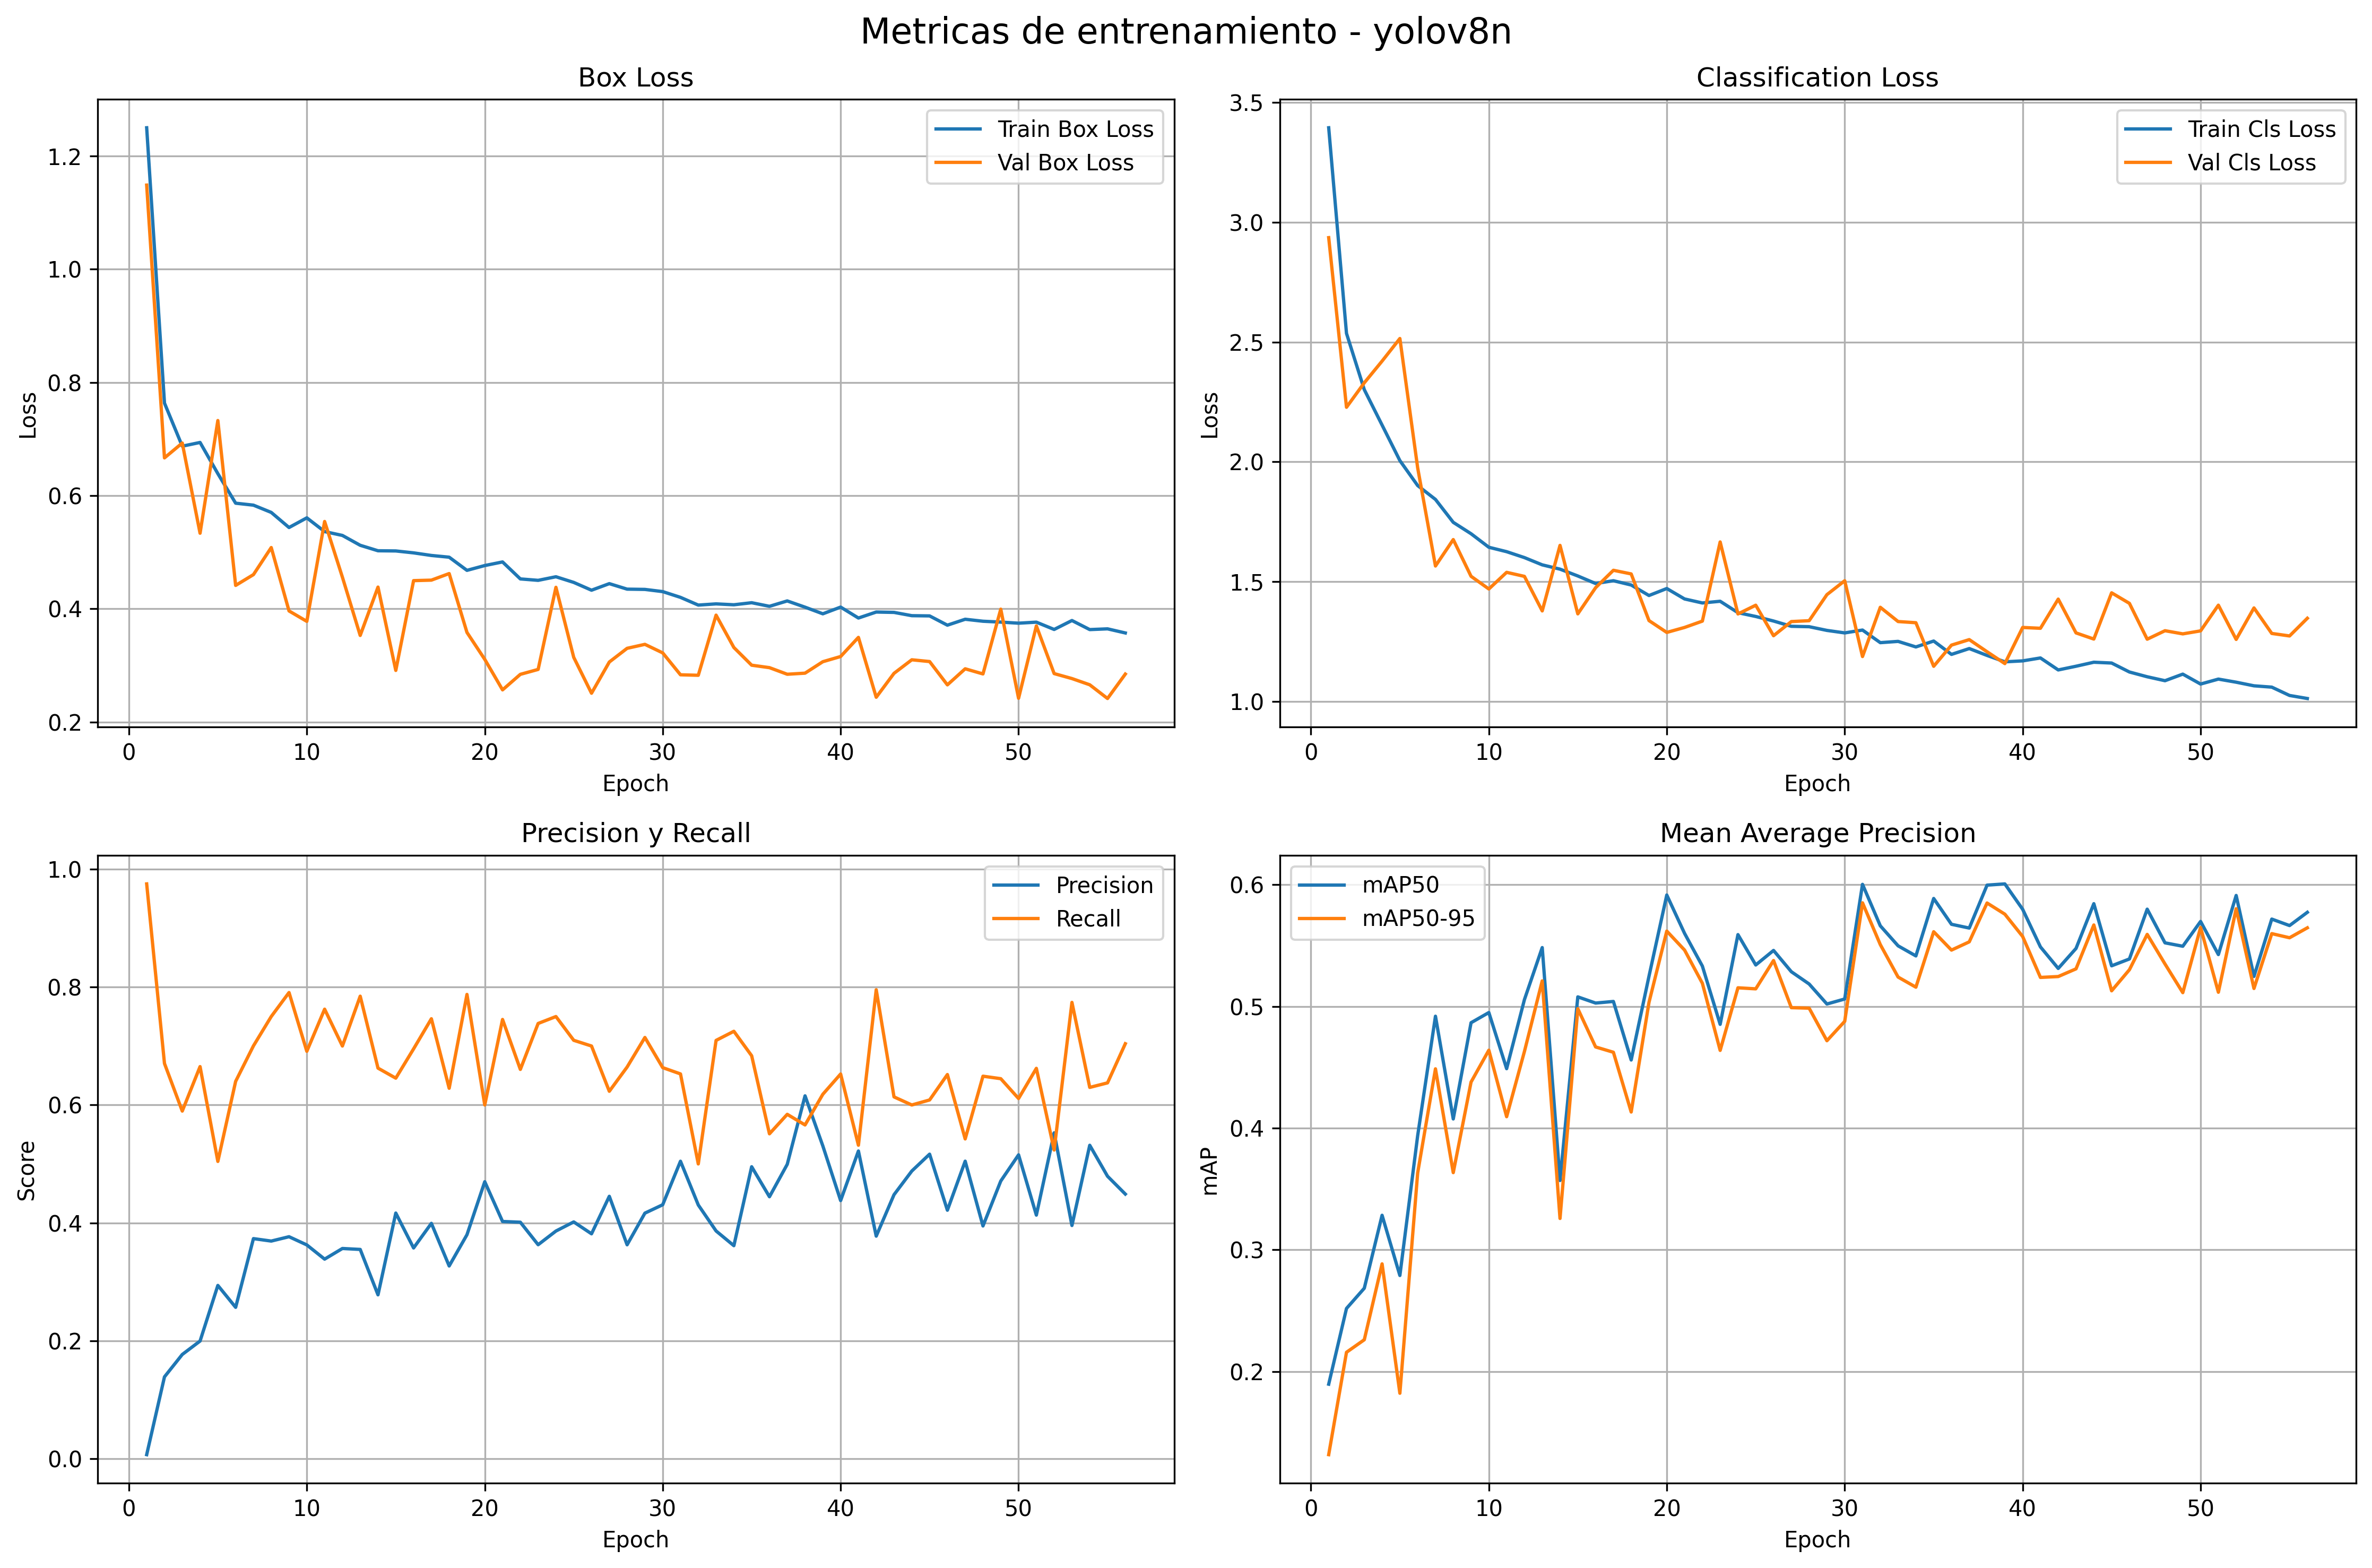
\includegraphics[width=\textwidth]{images/metrics_yolov8n.png}
\caption{Métricas de entrenamiento del modelo YOLOv8n. Se observa una disminución consistente de las funciones de pérdida y un incremento gradual de las métricas de evaluación a lo largo de las épocas de entrenamiento.}
\label{fig:training_yolov8n}
\end{figure}

La Figura~\ref{fig:training_yolov8s} presenta las métricas correspondientes al modelo YOLOv8s. Este modelo muestra un comportamiento similar al modelo nano, con una convergencia ligeramente más rápida en las primeras épocas. La pérdida de clasificación desciende de forma más pronunciada, lo que sugiere que la mayor capacidad del modelo le permite aprender patrones más discriminativos entre las diferentes clases de lesiones cutáneas. El modelo YOLOv8s completa aproximadamente 85 épocas antes de que el early stopping detenga el entrenamiento.

\begin{figure}[H]
\centering
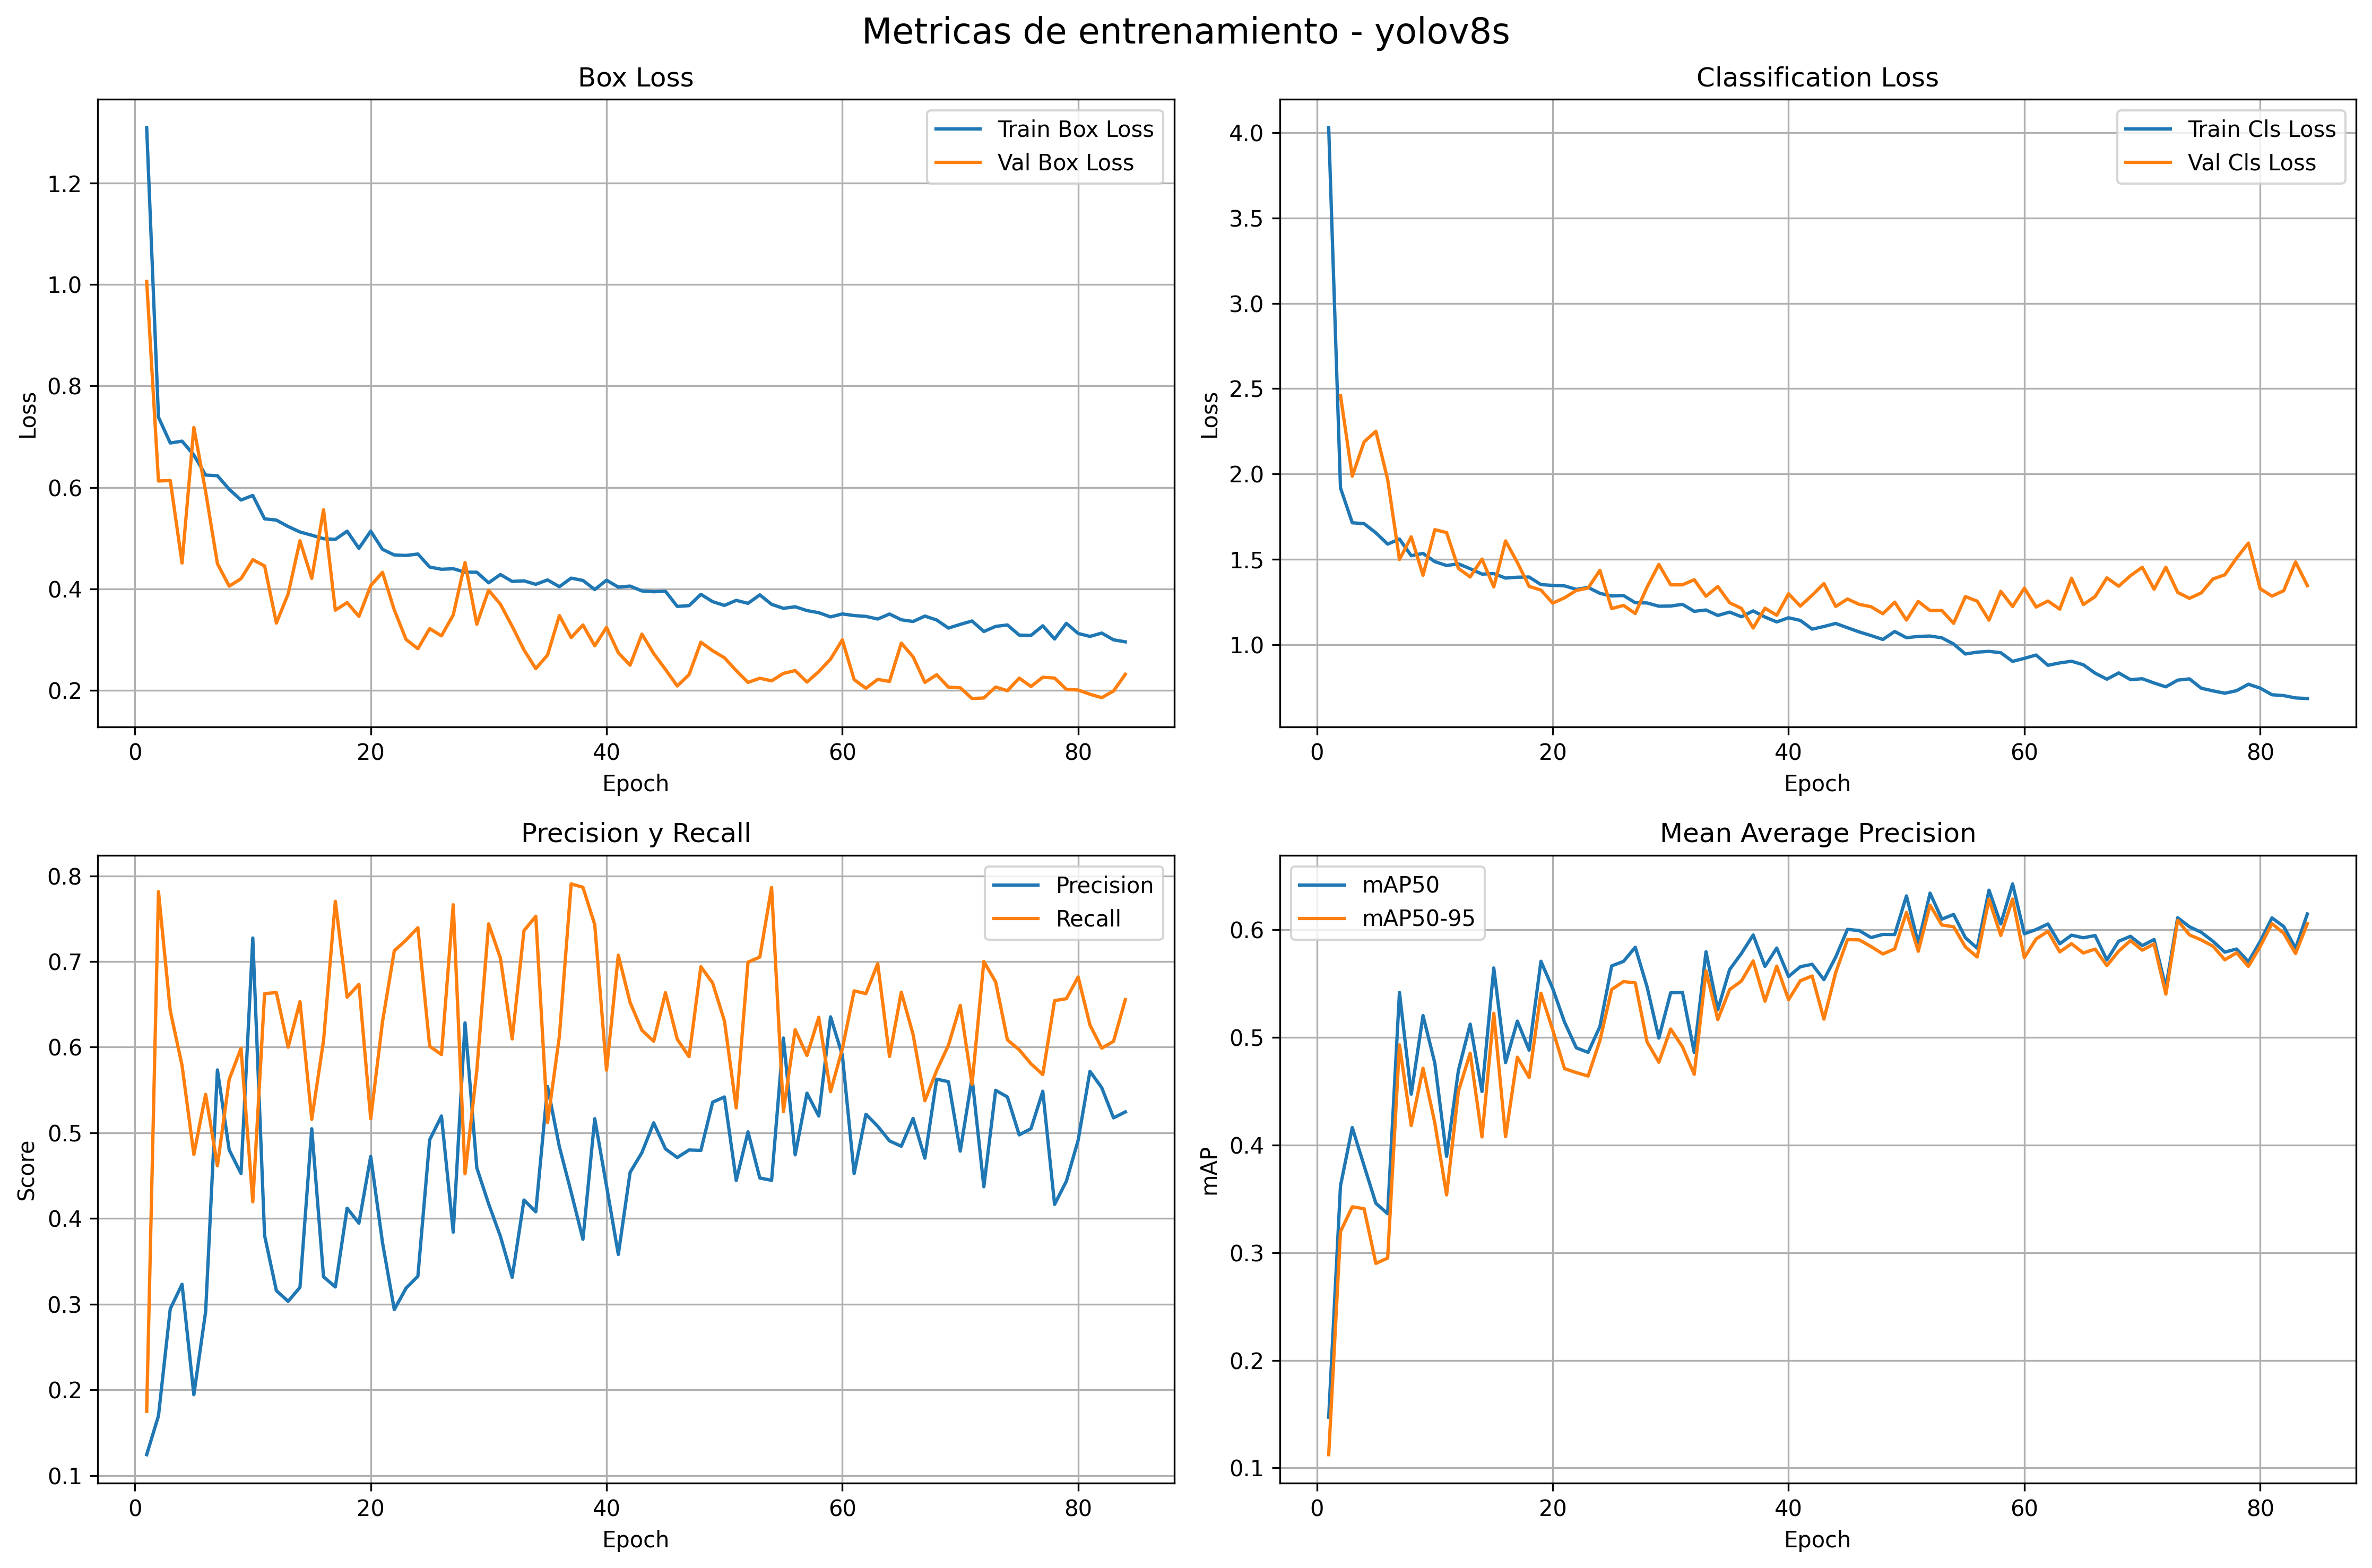
\includegraphics[width=\textwidth]{images/metrics_yolov8s.png}
\caption{Métricas de entrenamiento del modelo YOLOv8s. El modelo presenta una convergencia similar al YOLOv8n pero con valores finales de mAP ligeramente superiores.}
\label{fig:training_yolov8s}
\end{figure}

La Figura~\ref{fig:training_yolov8m} ilustra el proceso de entrenamiento del modelo YOLOv8m. Observamos que este modelo, al tener mayor capacidad, presenta picos más pronunciados en la pérdida de validación durante las primeras épocas, especialmente en el box loss y classification loss. Sin embargo, conforme avanza el entrenamiento, las curvas se estabilizan y el modelo alcanza los mejores valores de mAP entre los tres modelos evaluados. El entrenamiento completo del modelo medium consume significativamente más tiempo debido a su mayor número de parámetros.

\begin{figure}[H]
\centering
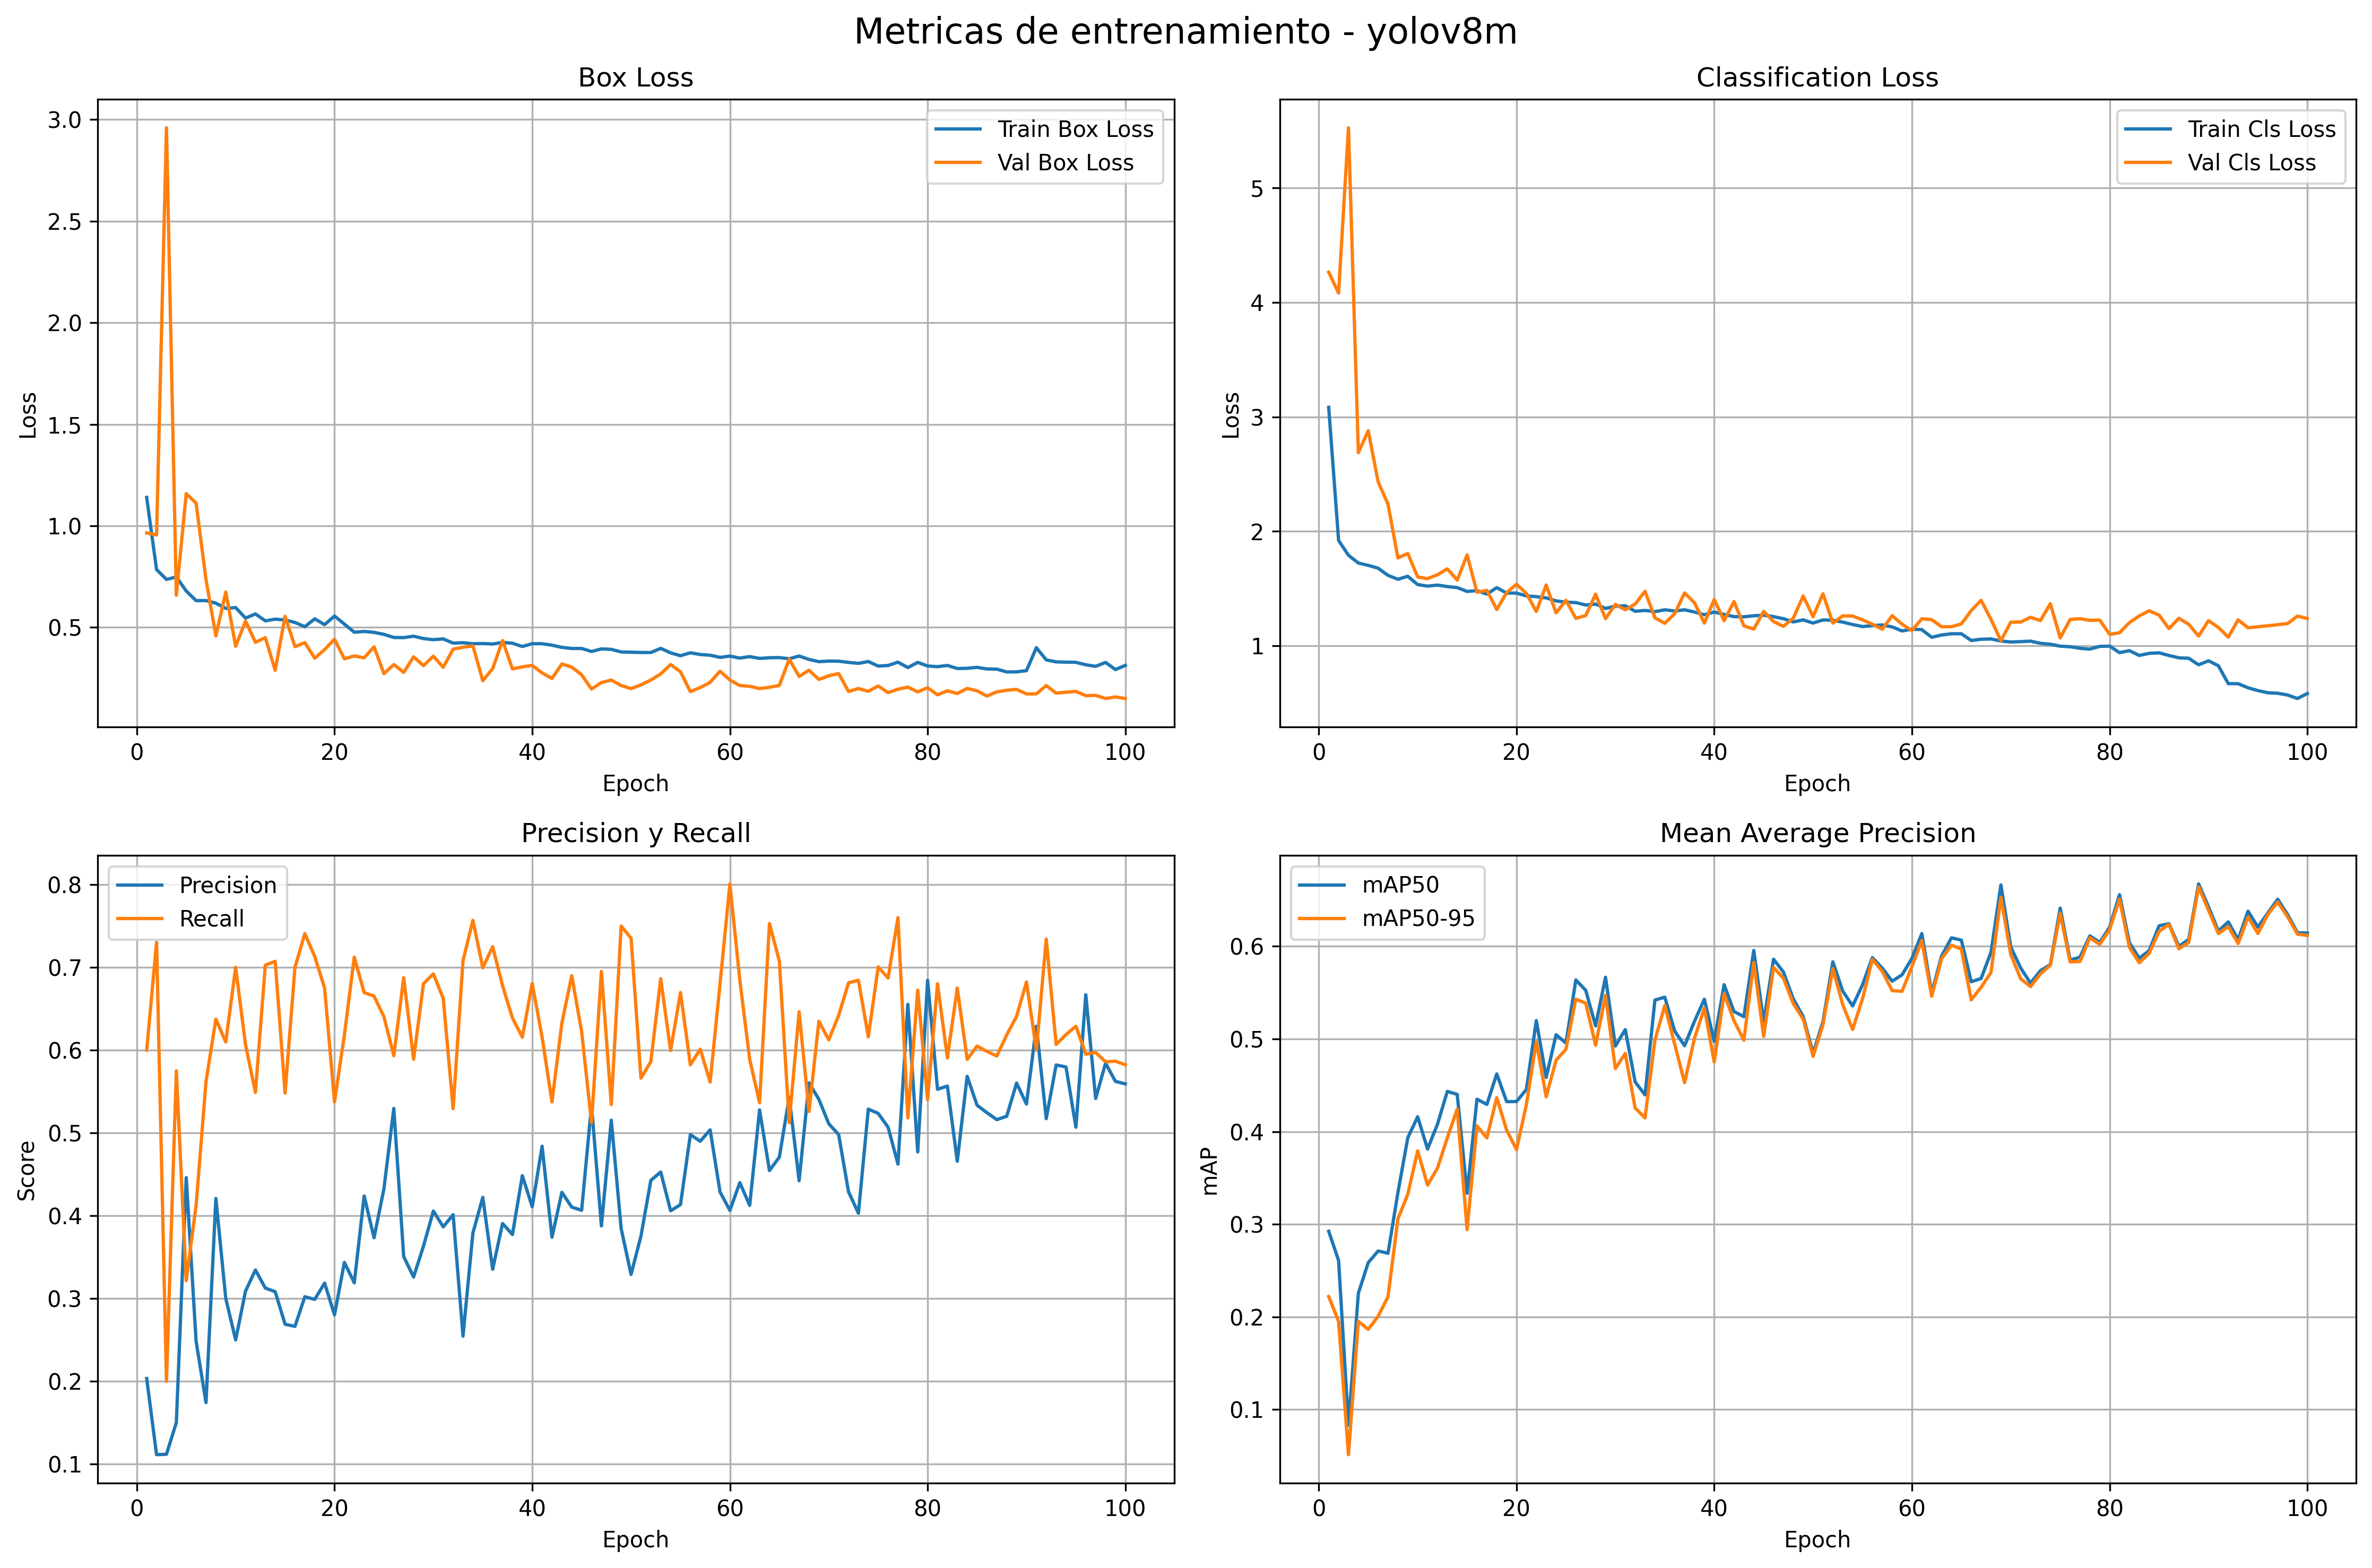
\includegraphics[width=\textwidth]{images/metrics_yolov8m.png}
\caption{Métricas de entrenamiento del modelo YOLOv8m. A pesar de mostrar mayor variabilidad inicial, este modelo alcanza los mejores valores finales de mAP.}
\label{fig:training_yolov8m}
\end{figure}

La Figura~\ref{fig:comparison_models} presenta una comparación directa entre los tres modelos en términos de pérdida de validación y mAP50. Podemos apreciar que los tres modelos convergen hacia valores similares de box loss al final del entrenamiento, aunque el modelo YOLOv8m presenta mayor inestabilidad inicial. En cuanto al mAP50, observamos que los tres modelos siguen trayectorias similares con una tendencia creciente, siendo el modelo YOLOv8m el que alcanza consistentemente los valores más altos a partir de la época 60 aproximadamente.

\begin{figure}[H]
\centering
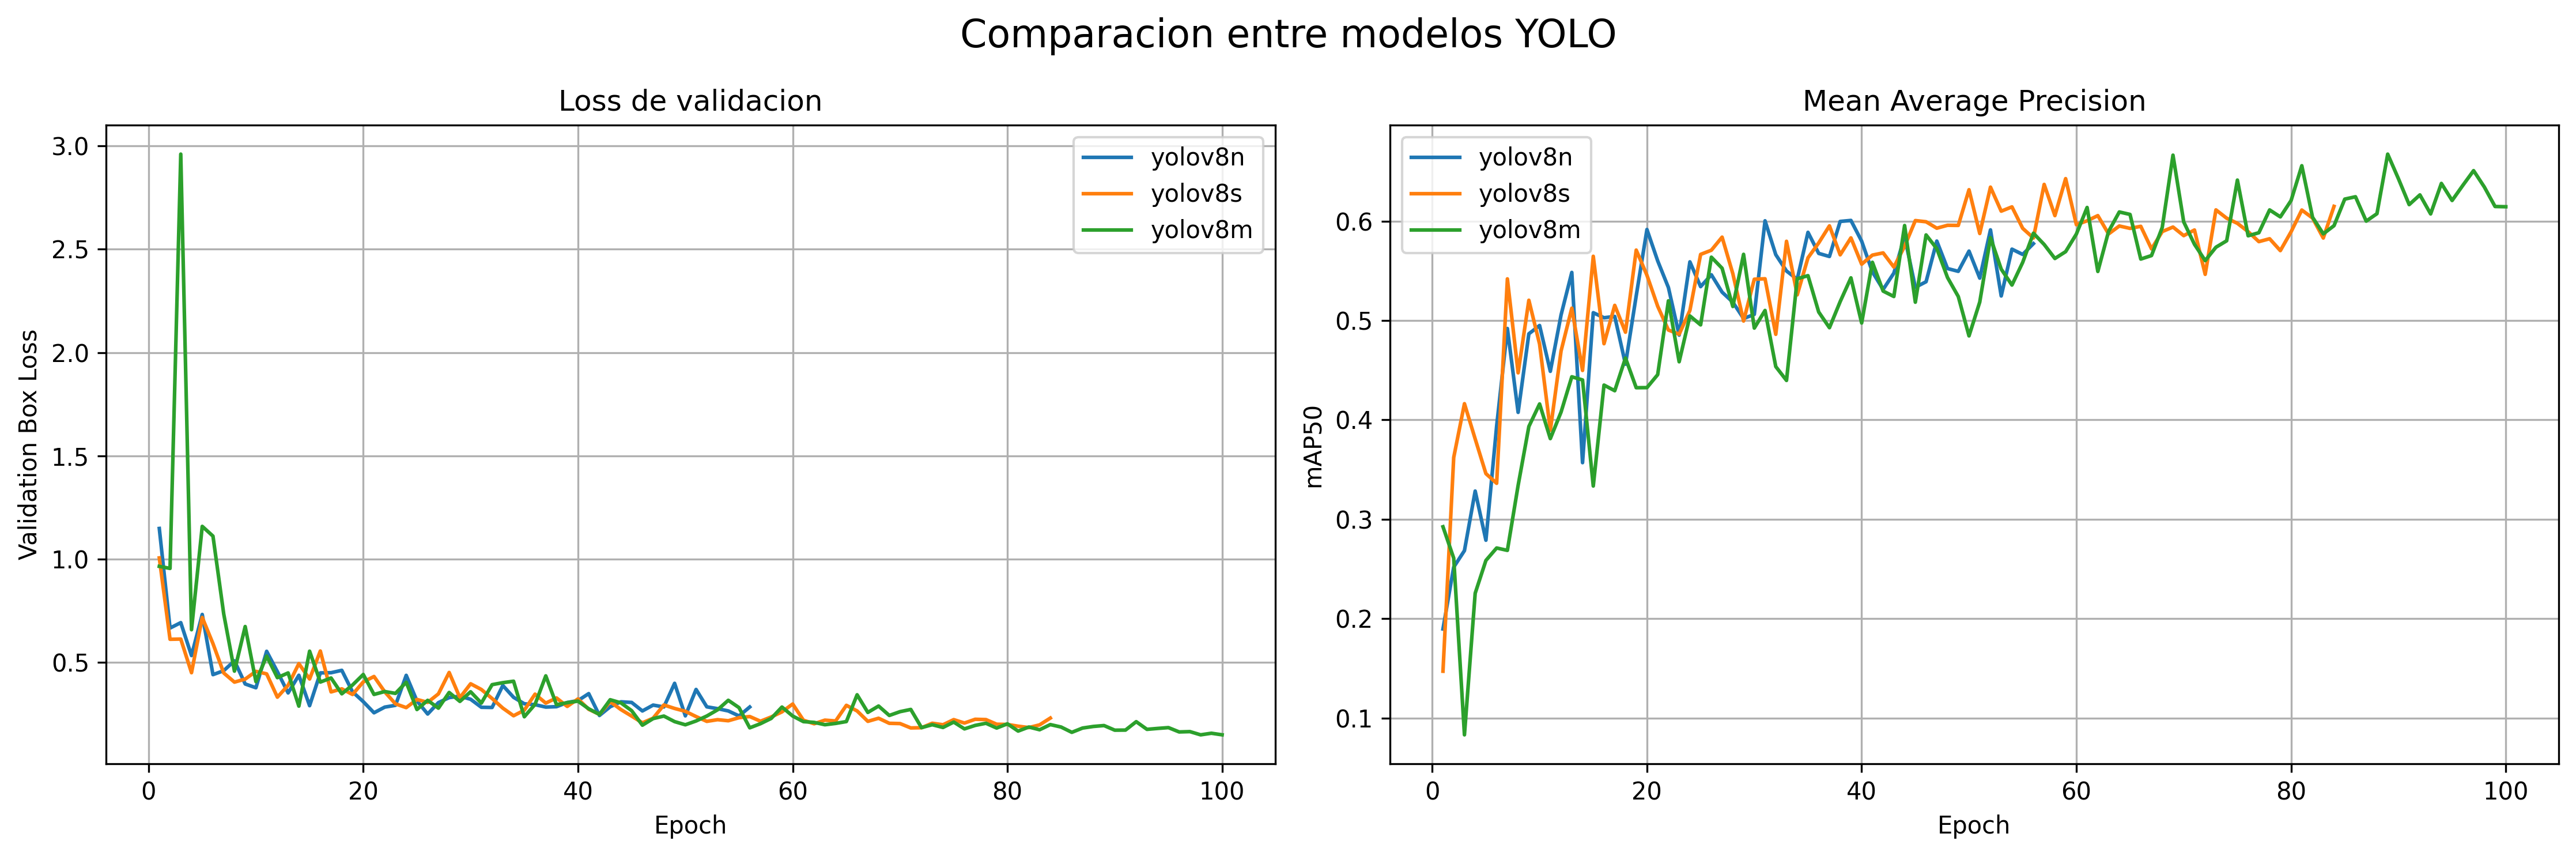
\includegraphics[width=\textwidth]{images/comparation_models.png}
\caption{Comparación entre los tres modelos YOLO durante el entrenamiento. Se muestra la evolución de la pérdida de validación y el mAP50 a lo largo de las épocas.}
\label{fig:comparison_models}
\end{figure}

\section{Evaluación y Resultados}

Una vez completado el entrenamiento de nuestros tres modelos, procedimos a evaluar su rendimiento en el conjunto de test que habíamos reservado previamente. Para cada modelo hemos calculado diversas métricas que nos permiten caracterizar su comportamiento desde diferentes perspectivas.

La Tabla~\ref{tab:model_results} resume las principales métricas de rendimiento obtenidas por cada modelo. El mAP50 (mean Average Precision con umbral IoU de 0.50) mide la precisión promedio de las detecciones cuando se considera que una predicción es correcta si el solapamiento entre el bounding box predicho y el real supera el 50\%. El mAP50-95 es una métrica más estricta que promedia el mAP calculado con umbrales IoU desde 0.50 hasta 0.95 en incrementos de 0.05. La Precision indica la proporción de detecciones positivas que son realmente correctas, mientras que el Recall mide la proporción de objetos reales que el modelo logra detectar. Finalmente, la Accuracy representa el porcentaje de clasificaciones correctas cuando asignamos a cada imagen la clase predicha por el modelo.

\begin{table}[H]
\caption{Comparativa de métricas de rendimiento para los tres modelos YOLO entrenados.}
\label{tab:model_results}
\centering
\begin{tabular}{lccccc}
\toprule
Modelo & mAP50 & mAP50-95 & Precision & Recall & Accuracy \\
\midrule
YOLOv8n & 0.608 & 0.594 & 0.509 & 0.652 & 0.507 \\
YOLOv8s & 0.650 & 0.636 & 0.550 & 0.634 & 0.633 \\
YOLOv8m & 0.664 & 0.661 & 0.563 & 0.647 & 0.582 \\
\bottomrule
\end{tabular}
\end{table}

Analizando los resultados de la Tabla~\ref{tab:model_results}, observamos que el modelo YOLOv8m obtiene los mejores valores en mAP50 (0.664), mAP50-95 (0.661) y Precision (0.563). Estos resultados confirman nuestra hipótesis de que los modelos más grandes, con mayor capacidad de representación, logran capturar patrones más sutiles en las imágenes de lesiones cutáneas. Sin embargo, resulta interesante notar que el modelo YOLOv8n alcanza el mejor Recall (0.652), lo que indica que el modelo más pequeño tiene una mayor tendencia a detectar lesiones, aunque con menor precisión. Por otro lado, el modelo YOLOv8s obtiene la mejor Accuracy en clasificación (0.633), sugiriendo que representa un buen equilibrio entre la capacidad de detección y la precisión en la asignación de clases.

La mejora de YOLOv8n a YOLOv8s representa un incremento del 7\% aproximadamente en mAP50 y mAP50-95, mientras que la mejora adicional de YOLOv8s a YOLOv8m es más modesta, cercana al 2\%. Este patrón de rendimientos marginales decrecientes es consistente con lo observado en otros dominios de aplicación de YOLO y sugiere que, para conjuntos de datos de tamaño limitado como el nuestro, los modelos más grandes no necesariamente proporcionan mejoras proporcionales a su incremento en complejidad.

La Figura~\ref{fig:confusion_matrices} muestra las matrices de confusión para cada uno de nuestros tres modelos. Estas matrices nos permiten visualizar qué tipos de errores comete cada modelo y cuáles son las clases más difíciles de clasificar correctamente.

\begin{figure}[H]
\centering
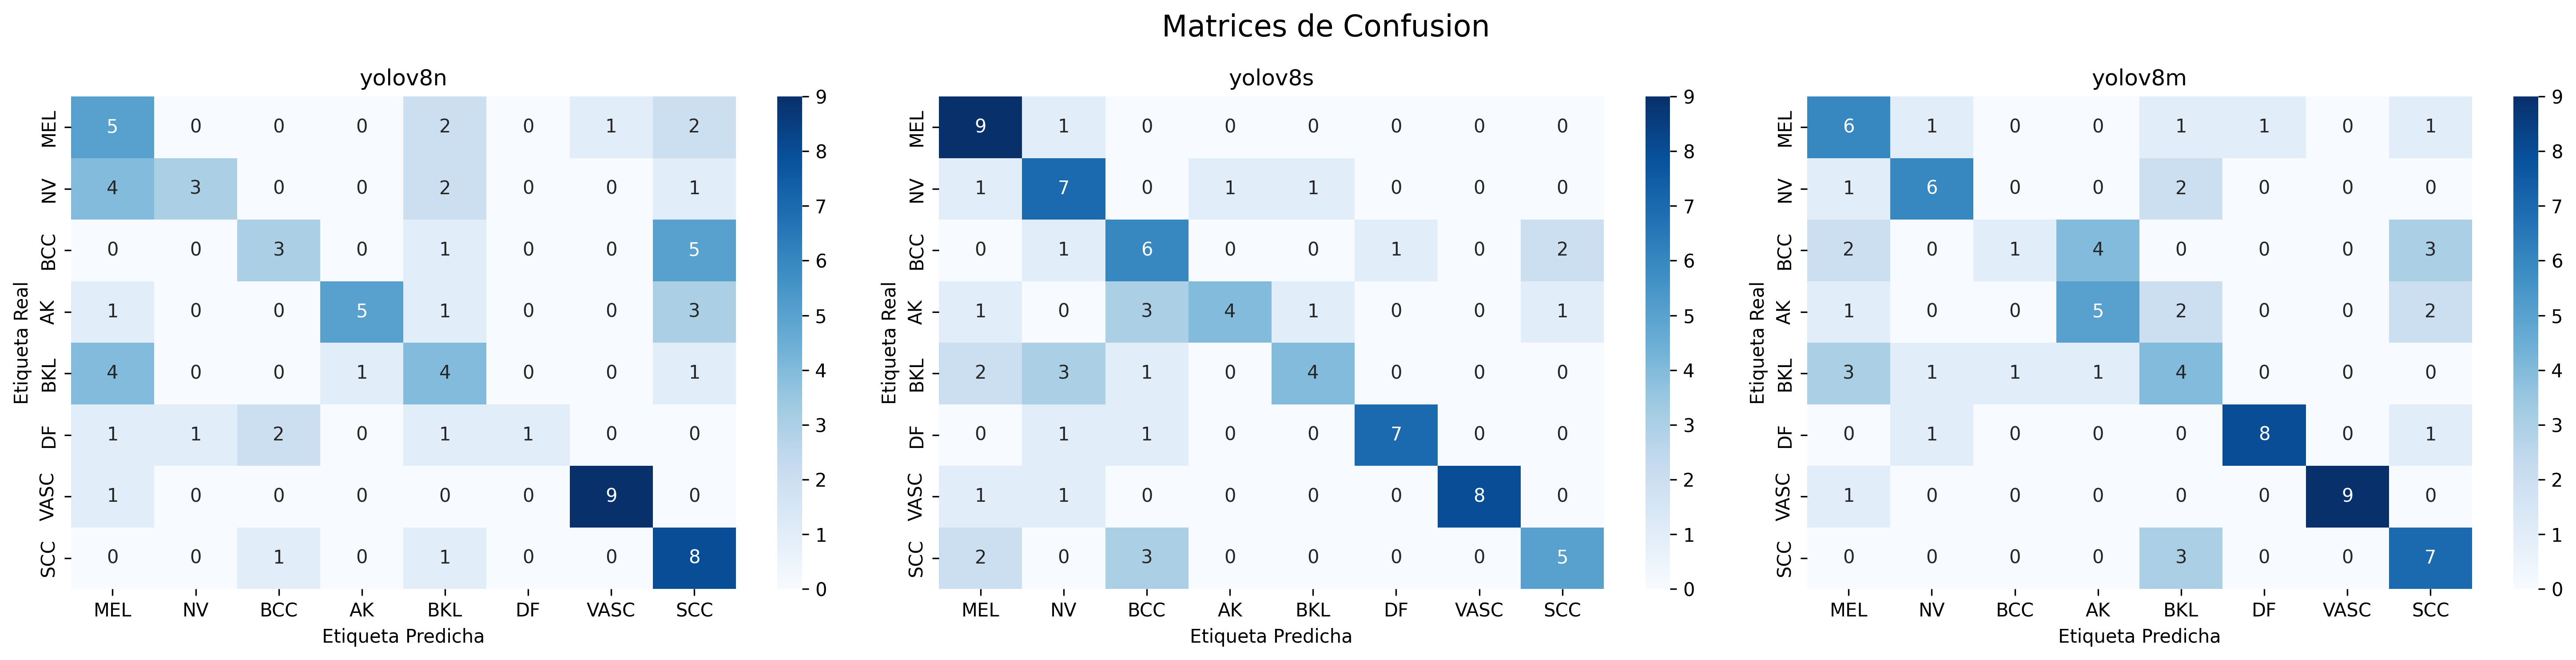
\includegraphics[width=\textwidth]{images/confusion_matrices.png}
\caption{Matrices de confusión para los tres modelos YOLO. Cada celda muestra el número de imágenes de la clase real (eje Y) que fueron clasificadas como la clase predicha (eje X).}
\label{fig:confusion_matrices}
\end{figure}

El análisis de las matrices de confusión revela varios patrones interesantes sobre el comportamiento de nuestros modelos. En primer lugar, observamos que las clases VASC (lesiones vasculares) y DF (dermatofibroma) son las que presentan mayor facilidad de clasificación, con la mayoría de los modelos alcanzando valores elevados en la diagonal principal para estas categorías. Esto puede explicarse por las características visuales distintivas de estas lesiones, que las hacen más fácilmente distinguibles del resto.

Por otro lado, las clases que presentan mayor confusión son MEL (melanoma), NV (nevus) y BCC (carcinoma basocelular). Estos tres tipos de lesiones comparten ciertas características morfológicas que dificultan su discriminación, lo cual representa un desafío clínico real en el diagnóstico dermatológico. Es particularmente preocupante la confusión entre melanoma y nevus, ya que el primero es una lesión maligna potencialmente mortal mientras que el segundo es benigno. Nuestros modelos muestran cierta tendencia a confundir estas categorías, lo que indica la necesidad de incorporar más datos de entrenamiento o técnicas adicionales de mejora en futuras iteraciones del sistema.

La comparación entre las tres matrices revela que el modelo YOLOv8s presenta la diagonal principal más marcada, lo que explica su mayor Accuracy global. El modelo YOLOv8m, aunque obtiene mejor mAP, distribuye sus errores de forma más uniforme entre las diferentes clases. El modelo YOLOv8n muestra mayor dispersión en sus predicciones, con valores más bajos en la diagonal para la mayoría de las clases.

\section{Análisis del Comportamiento durante el Entrenamiento}

El análisis de las curvas de entrenamiento nos permite evaluar si nuestros modelos presentan fenómenos de sobreajuste (overfitting) o subajuste (underfitting), aspectos fundamentales para determinar si el proceso de entrenamiento ha sido adecuado y si los modelos generalizarán correctamente a datos no vistos.

En el caso del sobreajuste, observaríamos que las métricas en el conjunto de entrenamiento continúan mejorando mientras que las métricas en el conjunto de validación se estancan o incluso empeoran. Este fenómeno indica que el modelo está memorizando los datos de entrenamiento en lugar de aprender patrones generalizables. En nuestros experimentos, las gráficas de las funciones de pérdida muestran que tanto la pérdida de entrenamiento como la de validación disminuyen de forma consistente y paralela a lo largo de las épocas, sin evidencia clara de divergencia. Esto sugiere que nuestros modelos no sufren de sobreajuste significativo.

El subajuste, por otro lado, se manifestaría si tanto las métricas de entrenamiento como las de validación mostraran valores pobres y sin tendencia clara de mejora. En nuestro caso, observamos una mejora constante en las métricas de mAP a lo largo del entrenamiento, lo que indica que nuestros modelos están aprendiendo efectivamente de los datos. Sin embargo, los valores finales de mAP alrededor de 0.60-0.66 sugieren que existe margen de mejora, posiblemente aumentando el tamaño del conjunto de entrenamiento o utilizando técnicas de data augmentation más agresivas.

Un aspecto notable en nuestras curvas de entrenamiento es la alta variabilidad de las métricas de Precision y Recall a lo largo de las épocas. Esta oscilación se debe en parte al pequeño tamaño de nuestro conjunto de validación (80 imágenes) y a la naturaleza del problema de clasificación multiclase con ocho categorías. Con conjuntos de datos más grandes, esperaríamos curvas más suaves y estables.

El sistema de early stopping implementado en nuestro entrenamiento con una paciencia de 25 épocas ha funcionado correctamente, deteniendo el entrenamiento cuando no se observan mejoras significativas en el rendimiento de validación. Esto nos ha permitido ahorrar tiempo de computación y evitar el sobreajuste que podría producirse si continuásemos entrenando indefinidamente.

\section{Conclusiones}

En este trabajo hemos desarrollado y evaluado un sistema de clasificación de lesiones cutáneas basado en aprendizaje profundo utilizando la arquitectura YOLOv8. Partiendo del conjunto de datos ISIC 2019, hemos creado subconjuntos balanceados de entrenamiento y test, y hemos entrenado tres variantes del modelo YOLO con diferentes niveles de complejidad.

Nuestros resultados demuestran que las arquitecturas basadas en YOLO pueden aplicarse de forma efectiva al problema de clasificación de lesiones cutáneas, alcanzando valores de mAP50 de hasta 0.664 con el modelo YOLOv8m. El análisis comparativo entre los tres modelos revela un compromiso claro entre complejidad computacional y rendimiento, donde el modelo medium obtiene las mejores métricas de detección mientras que el modelo small logra la mejor accuracy en clasificación.

El estudio de las curvas de entrenamiento nos ha permitido verificar que nuestros modelos aprenden de forma adecuada sin evidencia significativa de sobreajuste. Las funciones de pérdida de entrenamiento y validación evolucionan de forma paralela, y las métricas de evaluación mejoran consistentemente a lo largo del proceso de entrenamiento hasta alcanzar un punto de convergencia.

El análisis de las matrices de confusión ha revelado los principales desafíos de nuestro sistema, identificando las clases que presentan mayor dificultad de discriminación. Las lesiones vasculares y el dermatofibroma son clasificadas con alta precisión, mientras que el melanoma, el nevus y el carcinoma basocelular presentan mayor confusión entre sí, reflejando la dificultad inherente de distinguir estas lesiones incluso para especialistas humanos.

Como trabajo futuro, proponemos aumentar significativamente el tamaño del conjunto de entrenamiento para mejorar la capacidad de generalización de nuestros modelos. También consideramos la posibilidad de aplicar técnicas de data augmentation específicas para imágenes médicas y explorar arquitecturas alternativas como Vision Transformers. La incorporación de información clínica adicional, como la edad del paciente o la localización anatómica de la lesión, podría mejorar también el rendimiento del sistema.

Los resultados obtenidos en este proyecto demuestran el potencial del aprendizaje profundo para asistir en el diagnóstico de lesiones cutáneas, aunque es importante enfatizar que estos sistemas deben considerarse como herramientas de apoyo al diagnóstico clínico y no como sustitutos del criterio médico especializado.

\begin{thebibliography}{9}

\bibitem{yolov8}
Jocher, G., Chaurasia, A., \& Qiu, J. (2023).
\textit{Ultralytics YOLOv8}.
\url{https://github.com/ultralytics/ultralytics}

\bibitem{isic2019}
Combalia, M., et al. (2019).
\textit{BCN20000: Dermoscopic Lesions in the Wild}.
arXiv preprint arXiv:1908.02288.

\bibitem{tschandl2018}
Tschandl, P., Rosendahl, C., \& Kittler, H. (2018).
\textit{The HAM10000 dataset, a large collection of multi-source dermatoscopic images of common pigmented skin lesions}.
Scientific Data, 5, 180161.

\bibitem{esteva2017}
Esteva, A., et al. (2017).
\textit{Dermatologist-level classification of skin cancer with deep neural networks}.
Nature, 542(7639), 115-118.

\end{thebibliography}

\end{document}
